%%%%%%%%%%%%%%%%%%%%%%%%%%%%%%%%%%%%
%%%%%% AVERAGE 
%%%%%%%%%%%%%%%%%%%%%%%%%%%%%%%%%%%%
% Average % 5x5 % monolithic and all 
\begin{figure*}
\centering
\subfigure[5x5 Average Fitness]{
  \label{fig:esp_5x5_av_all}
  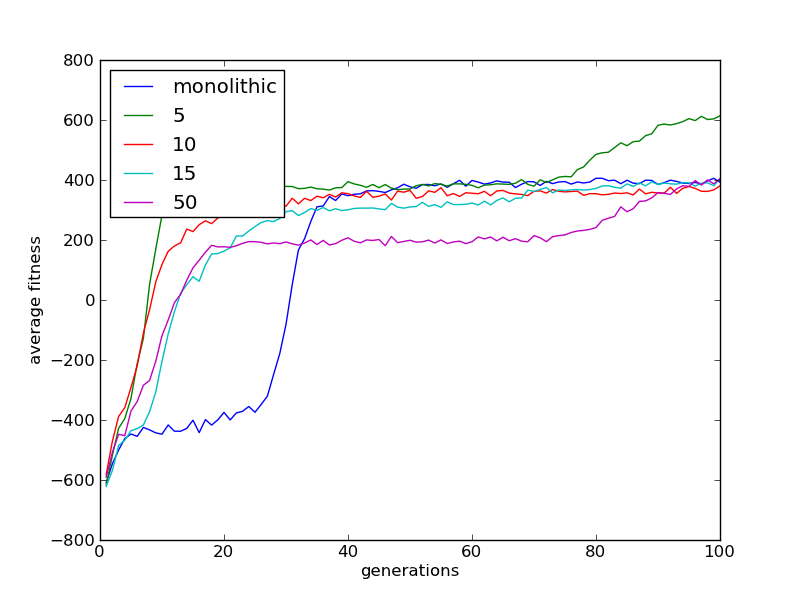
\includegraphics[scale=0.50]{figs/esp/fitness-vs-generations-5x5.png}}
\hspace{1in}
\subfigure[5x5 Percent Improvement]{
  \label{fig:esp_5x5_av_all_pi}
  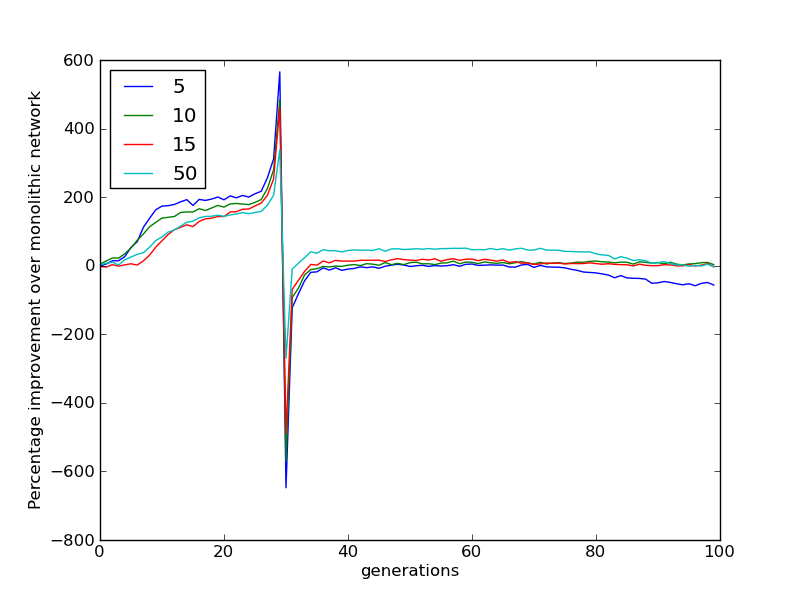
\includegraphics[scale=0.50]{figs/esp/improvement-vs-generations-5x5.png}}
  \caption{ESP: Average fitness plotted over generations for a 5x5 grid for
  monolithic network and network seeded with modular networks evolved for 5, 10, 15 and 50
  generations}
  \label{fig:MeanMAPNDCGPI9} % label for entire figure
\end{figure*}

% Average % 10x10 % monolithic and all 
\begin{figure*}
\centering
\subfigure[10x10 Average Fitness]{
  \label{fig:esp_10x10_av_all}
  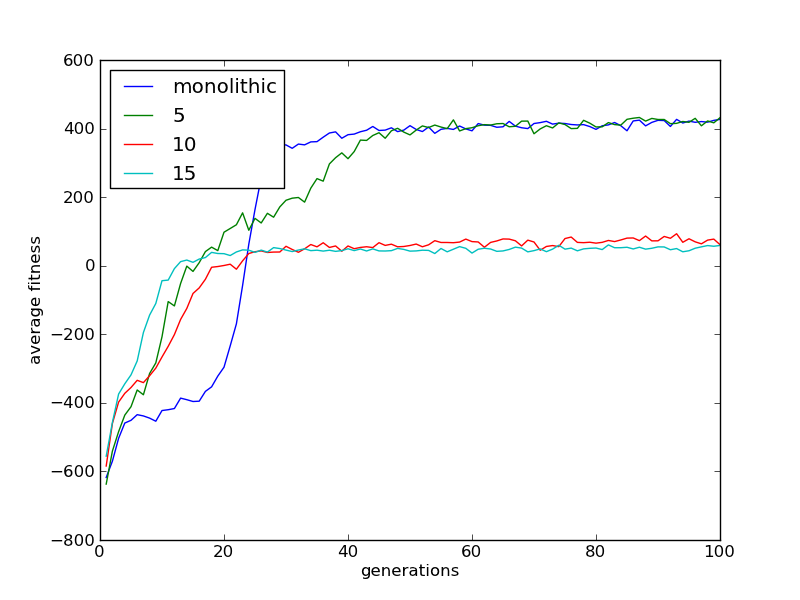
\includegraphics[scale=0.50]{figs/esp/fitness-vs-generations-10x10.png}}
\hspace{1in}
\subfigure[5x5 Percent Improvement]{
  \label{fig:esp_10x10_av_all_pi}
  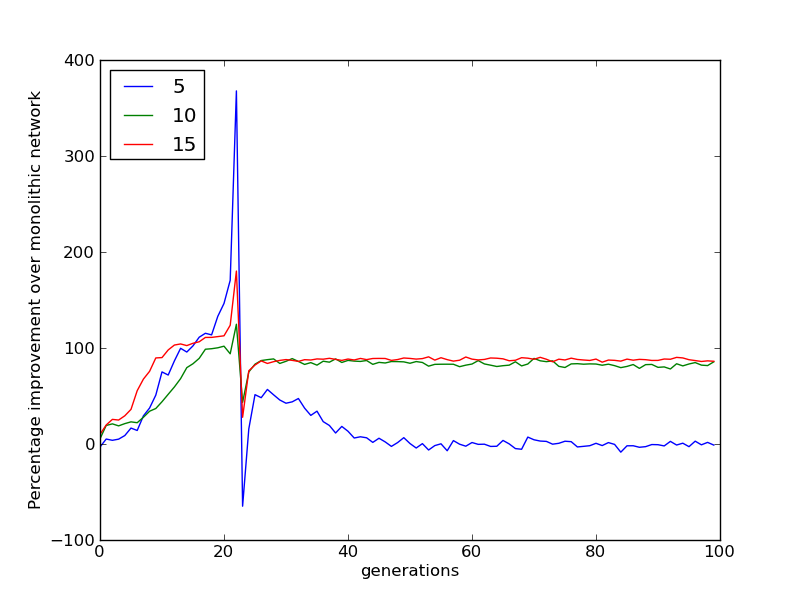
\includegraphics[scale=0.50]{figs/esp/improvement-vs-generations-10x10.png}}
  \caption{ESP: Average fitness plotted over generations for a 10x10 grid for
  monolithic network and network seeded with modular networks evolved for 5, 10, 15 and 50
  generations}
  \label{fig:MeanMAPNDCGPI10} % label for entire figure
\end{figure*}

% fitness-vs-generations-probs.png
%\begin{figure*}[htp]%
%	\centering
%	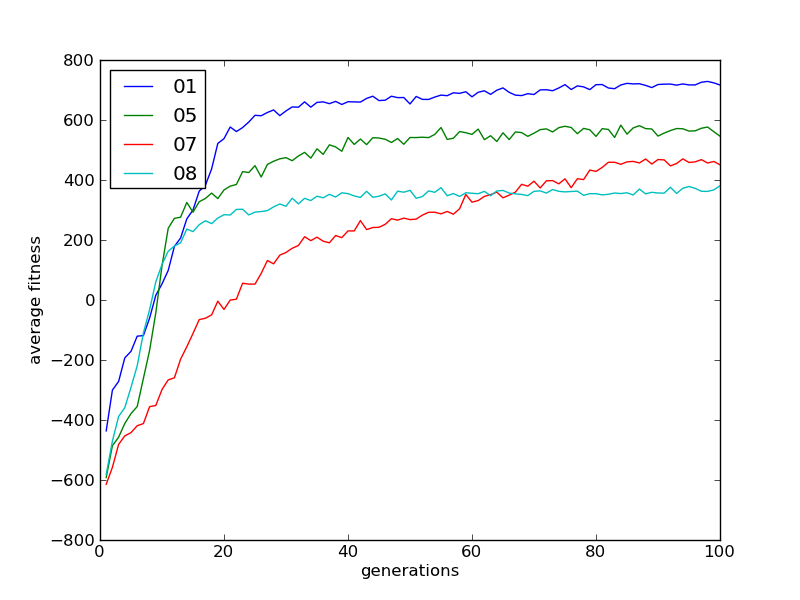
\includegraphics[scale=0.50]{figs/esp/fitness-vs-generations-probs.png}
%	\caption{Performance of modular approach on a 5x5 grid with different move probabilities (0.1, 0.5, 0.7, 0,8) of hunter and prey (values for both are set to be the same)}
%	\label{fig:MAPPIAll11}
%\end{figure*}
